\chapter{Геометрия, информация и закон площади чёрной дыры}

\lectureoverview{Заявленная цель — космология, но кратчайший путь к ней начинается с возвращения к специальной теории относительности. Метрика задаёт геометрию пространства-времени, а условие нулевого собственного времени говорит, как распространяется свет. Мы перенесём это единственное правило в геометрию Шварцшильда, отличим горизонт от сингулярности, а затем спросим, что происходит с информацией, когда чёрная дыра испаряется. Ответ начинается с обычной энтропии и заканчивается однобитным аргументом Бекенштейна: чёрная дыра хранит информацию в единицах площади горизонта, а не объёма.}

Сасскинд ненадолго откладывает обещанное подведение баланса успехов и неудач теории струн. Уже поздно, говорит он, и содержание полезнее, чем такой баланс. Сегодня речь пойдёт о минимуме геометрии и термодинамики, необходимом для формулировки проблемы информации в чёрной дыре.

\section{Одно правило для света}

Специальная теория относительности рассматривает пространство и время как единый геометрический объект. Для соседних событий, разделённых смещениями \(dt,dx,dy,dz\), Сасскинд использует сигнатуру с одним плюсом и тремя минусами и пишет
\begin{equation}
d\tau^2=dt^2-\frac{1}{c^2}\left(dx^2+dy^2+dz^2\right).
\end{equation}
Противоположные знаки временной и пространственной частей отличают геометрию Минковского от четырёхмерной евклидовой геометрии. Множитель \(1/c^2\) лишь согласует единицы измерения; выбрав согласованные единицы времени и расстояния, можно положить \(c=1\).

Для времениподобного интервала выполняется \(d\tau^2>0\), а \(d\tau\) — это собственное время, отсчитываемое часами, движущимися вдоль траектории. Пространственноподобные интервалы, напротив, характеризуются \(d\tau^2<0\). Случай, нужный нам сегодня, лежит точно между ними. Световой луч движется по \emph{нулевой} траектории,
\begin{equation}
d\tau^2=0.
\end{equation}
Если сначала ограничиться движением вдоль оси \(x\), получаем
\begin{align}
0&=dt^2-\frac{dx^2}{c^2},\\
c\,dt&=\pm dx,\\
\frac{dx}{dt}&=\pm c.
\end{align}
Знаки соответствуют лучам, распространяющимся вправо и влево. Численное значение, приписываемое \(c\), меняется, если заменить сантиметры метрами или километрами; инвариантным утверждением является не число, а нулевое условие.

Общая теория относительности усложняет метрику, но не это правило. В координатах \(x^\mu\), \(\mu=0,1,2,3\),
\begin{equation}
ds^2=g_{\mu\nu}(x)\,dx^\mu dx^\nu,
\end{equation}
где по повторяющимся индексам производится суммирование, а коэффициенты могут меняться от точки к точке. Чтобы найти локально допустимые направления распространения света, нужно приравнять эту квадратичную форму к нулю.

\section{Сферические координаты и метрика Шварцшильда}

Невращающаяся чёрная дыра сферически симметрична, поэтому декартовы координаты скрывают полезную структуру. Пусть \(r\) измеряет радиальное расстояние, а \(\theta,\phi\) задают направление на единичной сфере. Её линейный элемент имеет вид
\begin{equation}
d\Omega^2=d\theta^2+\sin^2\theta\,d\phi^2.
\end{equation}
Поэтому на сфере радиуса \(r\) угловые смещения дают вклад \(r^2d\Omega^2\). Плоское пространство-время в сферических координатах записывается так:
\begin{equation}
d\tau^2=dt^2-\left(dr^2+r^2d\Omega^2\right),
\qquad (c=1).
\end{equation}

Сасскинд не выводит решение для чёрной дыры из уравнений Эйнштейна. Он просто выписывает его и предлагает нам его рассмотреть. На доске явно показано, с чем его следует сравнивать.

\begin{figure}[htbp]
\centering
\includegraphics[width=0.86\textwidth]{lecture_02_figure_02.png}
\caption{Плоское сферическое пространство-время над шварцшильдовской деформацией. Повторяющийся множитель \(1-2GM/(c^2r)=1-R_s/r\) и радиальный набросок видны одновременно.}
\lectureframe{00:19:12.520}
\end{figure}

Для чёрной дыры массы \(M\) определим радиус Шварцшильда
\begin{equation}
R_s=\frac{2GM}{c^2}.
\end{equation}
Внешний линейный элемент имеет вид
\begin{equation}
d\tau^2=\left(1-\frac{R_s}{r}\right)dt^2
-\frac{dr^2/c^2}{1-R_s/r}
-\frac{r^2}{c^2}d\Omega^2.
\label{eq:schwarzschild-explicit-c}
\end{equation}
Эквивалентно, если положить \(c=1\),
\begin{equation}
ds^2=\left(1-\frac{2GM}{r}\right)dt^2
-\frac{dr^2}{1-2GM/r}-r^2d\Omega^2.
\label{eq:schwarzschild}
\end{equation}
Вдали, где \(R_s/r\ll1\), восстанавливается плоская сферическая метрика. Эта асимптотическая проверка важнее, чем заучивание формулы, хотя Сасскинд рекомендует последнее как материал для разговоров на коктейльных вечеринках.

\editorialnote{На доске чередуются \(d\tau^2\) и \(ds^2\), и не каждый множитель \(c\) выписан согласованно. Уравнение~\eqref{eq:schwarzschild-explicit-c} следует принятому в лекции соглашению о временной координате, в котором \(t\) имеет размерность времени. Стандартная форма с \(x^0=ct\) алгебраически эквивалентна.}

\subsection{Горизонт — не сингулярность}

В координатах подозрительно выглядят два радиуса. При \(r=R_s=2GM\) в натуральных единицах коэффициент при \(dt^2\) обращается в нуль, а коэффициент при \(dr^2\) расходится. При \(r=0\) сингулярной становится сама кривизна. Это не две версии одного и того же события:
\begin{equation}
\begin{aligned}
r=R_s &:\quad \text{horizon},\\
r=0 &:\quad \text{curvature singularity}.
\end{aligned}
\end{equation}

Приливные силы дают физическое различие. Гравитационное поле меняется по протяжённому телу: ноги могут притягиваться сильнее, чем голова, растягивая тело, тогда как поперечные направления сжимаются. На горизонте эти приливные силы конечны, а на горизонте достаточно массивной чёрной дыры они могут быть очень малы. Локально там вовсе не обязано происходить ничего катастрофического. Напротив, при \(r=0\) приливные силы расходятся. Тревожные коэффициенты при \(r=R_s\) указывают на дефект координат Шварцшильда; сингулярность при \(r=0\) физическая.

\editorialnote{Конечность кривизны при \(r=R_s\) можно проверить по скаляру Кретчмана \(R_{\mu\nu\rho\sigma}R^{\mu\nu\rho\sigma}=48G^2M^2/(c^4r^6)\), который конечен на горизонте и расходится только при \(r\to0\). Этот инвариант в лекции не был записан, но он точно формулирует это различие по приливным силам.}

\section{Радиальные световые лучи вблизи горизонта}

Теперь вернёмся к одному правилу. Радиальный луч идёт при фиксированных угловых координатах, поэтому \(d\Omega=0\), а для светового луча \(ds^2=0\). В единицах с \(c=1\) уравнение~\eqref{eq:schwarzschild} даёт
\begin{equation}
0=\left(1-\frac{2GM}{r}\right)dt^2
-\frac{dr^2}{1-2GM/r}.
\end{equation}
Умножение на \(1-2GM/r\) и извлечение квадратного корня дают две ветви,
\begin{align}
dr&=\pm\left(1-\frac{2GM}{r}\right)dt,\\
\frac{dr}{dt}&=\pm\left(1-\frac{2GM}{r}\right).
\label{eq:radial-null}
\end{align}
Знак плюс соответствует исходящему лучу, а знак минус — входящему. Вдали их координатные скорости стремятся к \(\pm1\). На горизонте для обоих выполняется \(\lvert dr/dt\rvert\to0\): в шварцшильдовом координатном времени исходящий луч кажется там неподвижным, тогда как входящему лучу требуется бесконечное координатное время, чтобы его достичь.

\begin{figure}[htbp]
\centering
\includegraphics[width=0.82\textwidth]{lecture_02_figure_03.png}
\caption{Завершённый набросок на доске в координатах \(t\)-\(r\): радиальные нулевые лучи становятся почти вертикальными по мере приближения к пунктирному горизонту.}
\lectureframe{00:30:25.000}
\end{figure}

\begin{figure}[htbp]
\centering
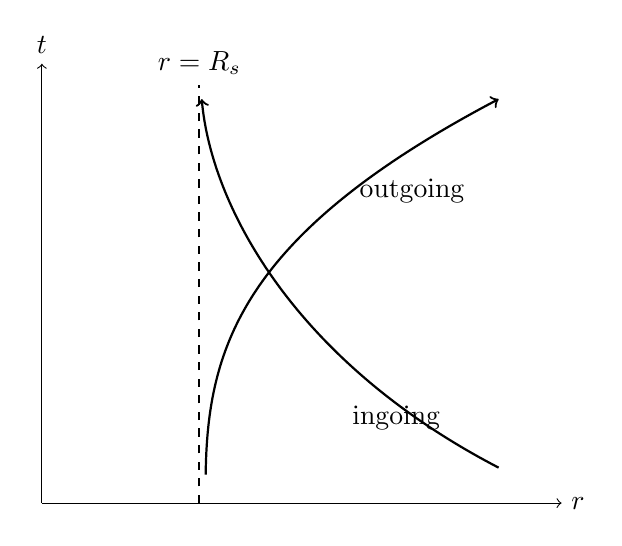
\begin{tikzpicture}[x=1.0cm,y=0.9cm]
\draw[->] (0,0) -- (6.6,0) node[right] {$r$};
\draw[->] (0,0) -- (0,6.2) node[above] {$t$};
\draw[dashed,thick] (2.0,0) -- (2.0,5.9) node[above] {$r=R_s$};
\draw[thick,->] (2.08,.4) .. controls (2.10,2.2) and (2.55,3.8) .. (5.8,5.7);
\draw[thick,->] (5.8,.5) .. controls (3.2,2.0) and (2.15,4.2) .. (2.03,5.7);
\node[align=center] at (4.7,4.4) {outgoing};
\node[align=center] at (4.5,1.2) {ingoing};
\end{tikzpicture}
\caption{Аккуратно перерисованный вариант наброска на доске в координатном времени. Кажущееся замедление относится к шварцшильдовской координате времени \(t\), а не к локальному нарушению движения света со скоростью \(c\).}
\end{figure}

Внутри горизонта световые конусы будущего наклоняются настолько внутрь, что обе направленные в будущее радиальные ветви ведут к уменьшению \(r\). Никакой сигнал, возникающий там, не может выйти во внешнюю область, и всякая направленная в будущее причинная траектория достигает сингулярности.

\begin{classroomqa}
\audiencequestion{Если скорость света инвариантна, то что именно означает утверждение, что вблизи горизонта свет замедляется?\lecturetimestamp{00:31:44}}
\lecturerresponse{Показанная величина — это \(dr/dt\) в некоторой системе координат. Численное значение скорости меняется уже при замене метров на сантиметры; здесь эффективные масштабы по радиусу и по времени зависят от положения. Универсальное утверждение состоит в том, что любой световой луч следует нулевой траектории, \(ds^2=0\).}
\end{classroomqa}
\editorialnote{Свободно падающий локальный наблюдатель измеряет для света в вакууме скорость \(c\); обращение в нуль шварцшильдовской координатной скорости на горизонте не является локально наблюдаемой величиной.}

\begin{classroomqa}
\audiencequestion{Сохраняется ли то же утверждение о светоподобном распространении независимо от материальной среды, через которую распространяется свет?\lecturetimestamp{00:33:24}}
\lecturerresponse{Нет. В доступной расшифровке более развёрнутое объяснение этого ответа не сохранилось.}
\end{classroomqa}
\editorialnote{Утверждение о светоподобном распространении относится к распространению в вакуумном пространстве-времени. Взаимодействия с веществом могут придавать волновому пакету меньшую эффективную скорость; это свойство среды, а не изменение локальной причинной скорости \(c\).}

\begin{classroomqa}
\audiencequestion{Как выглядит входящий световой луч на той же диаграмме \(t\)-\(r\)?\lecturetimestamp{00:33:32}}
\lecturerresponse{Это ветвь, выглядящая противоположным образом: начиная с больших \(r\), она изгибается к горизонту и асимптотически к нему приближается. Чтобы достичь его, требуется бесконечное координатное время \(t\).}
\end{classroomqa}
\editorialnote{Падающий наблюдатель достигает горизонта и пересекает его за конечное собственное время; расходится только шварцшильдово \(t\).}

\section{Почему испарение создаёт проблему}

Горизонт заслуживает гораздо более подробного изучения: как он формируется, что видит падающий наблюдатель и происходит ли там локально что-либо необычное. Сасскинд откладывает эти вопросы и переходит к квантовой механике. Снаружи вещество и вся информация, позволяющая его различать, всё теснее прижимаются к горизонту и становятся недоступными. Само по себе это не обязательно уничтожает информацию; оно может просто скрывать её.

Результат Хокинга делает этот вопрос особенно острым. Стационарная классическая черная дыра выглядит самым скучным объектом, какой только можно вообразить: сферическая, темная и не способная передать сообщение. Но слово ``черная'' имеет два значения. Оно может означать, что ничего не излучается, а может — что испускается тепловое излучение абсолютно черного тела. Квантовая черная дыра черна во втором смысле. У нее есть температура, она светится и теряет энергию. Поскольку
\begin{equation}
E=Mc^2,
\qquad
R_s=\frac{2GM}{c^2},
\end{equation}
излучение уменьшает и ее массу, и радиус горизонта. Если испарение в конце концов устранит дыру, что станет с информацией, которая, как казалось, оставалась на ее горизонте? Она может быть уничтожена, заключена в крошечном остатке или закодирована в исходящем излучении. Напряжение между этими возможностями и образует информационную проблему, и позднее теория струн поможет уточнить ее разрешение.

Сегодня вечером мы не будем пытаться вычислять квантовые поля в искривленном пространстве-времени. Вместо этого Сасскинд идет по более простому пути Бекенштейна: сначала понять энтропию как информацию, а затем вычислить, сколько информации может скрыть черная дыра.

\section{Информация, которая присутствует, но скрыта}

Представьте, что ящик разделен на настолько мелкие ячейки, что каждая ячейка либо занята, либо пуста. Двоичная строка---по одному ответу на ячейку---отличает данную конфигурацию от любой другой допустимой конфигурации. Для более реалистичной материи нужны вопросы о видах частиц и других степенях свободы, но принцип не меняется: информация измеряется минимальным числом вопросов типа да--нет, необходимых для задания состояния.

\begin{classroomqa}
\audiencequestion{Это только описание статической системы?\lecturetimestamp{00:45:49}}
\lecturerresponse{Это мгновенное описание, относящееся к одному моменту времени. Затем динамика отображает его в другое состояние.}
\end{classroomqa}

Следующий принцип глубже: эволюция замкнутой системы не сливает два различных микроскопических состояния в одно. Если две конфигурации различаются сейчас, то и их конфигурации после эволюции в принципе остаются различимыми. Классическая гамильтонова эволюция обратима, а квантовая эволюция унитарна.\editorialnote{Диссипативные эффективные уравнения могут стирать различия лишь потому, что ненаблюдаемые степени свободы окружения были опущены; полное состояние замкнутой системы их сохраняет.}

Пример с ванной наглядно показывает разницу между потерей и недоступностью. Два потока капель могли бы кодировать два разных сообщения азбукой Морзе. После того как вода успокоится, обе ванны будут выглядеть одинаково. Видимая рябь исчезнет, однако полное микроскопическое измерение все еще обнаружило бы разные молекулярные конфигурации. Сообщение рассеялось по степеням свободы, слишком малым и многочисленным, чтобы их отслеживать.

Энтропия и есть эта скрытая информация. С точки зрения макроскопических вопросов, которые мы можем задать---температура, полная энергия, состав, уровень воды---многие микроскопические различия остаются возможными, но недоступными. На языке подсчета битов, используемом в лекции,
\begin{equation}
S=\hbox{number of hidden bits}.
\end{equation}
Точная статистическая формула имеет вид \(S=k_B\ln\Omega\), но для аргумента о черной дыре достаточно и качественного определения.

\section{Температура как цена сокрытия одного бита}

Температуру привычно измерять, но определить ее оказывается на удивление непрямо. Сасскинд выбирает энтропию и энергию в качестве исходных понятий. Предположим, что компьютерный бит сбрасывается к стандартному значению. Физическое устройство остается, но различие между его прежними состояниями нуля и единицы исчезает из компьютера. Оно не может исчезнуть из мира в целом; оно переносится в микроскопические степени свободы окружения, которые из-за этого немного нагреваются. Это и есть принцип Ландауэра.

Если принять одну единицу энтропии за один бит, а температуру измерять в единицах энергии, то в лекции записывается
\begin{align}
\Delta S&=1,\\
\Delta E&=T\,\Delta S,\\
dE&=T\,dS.
\label{eq:first-law}
\end{align}

\begin{figure}[htbp]
\centering
\includegraphics[width=0.84\textwidth]{lecture_02_figure_04.png}
\caption{Информационно-теоретическая термодинамика на доске: \(S\) — это энтропия, один скрытый бит имеет \(\Delta S=1\), а его минимальная энергетическая цена записывается как \(\Delta E=T\Delta S\).}
\lectureframe{00:58:40.000}
\end{figure}

\editorialnote{В обычных единицах обратимая цена стирания одного двоичного бита равна \(k_BT\ln2\). Уравнение~\eqref{eq:first-law} использует \(k_B=1\) и считает, что единица энтропии в лекции равна одному биту, опуская связанный с этим \(\ln2\). Эти соглашения не влияют на последующий аргумент о масштабной зависимости.}

Оценка из аудитории дает для минимального повышения температуры стакана воды при стирании примерно \(100\) гигабайт величину порядка \(10^{-15}\) градусов. Сасскинд принимает саму суть, а не точное число: при комнатной температуре одному биту соответствует чрезвычайно малая минимальная энергия, а реальные компьютеры рассеивают гораздо больше, потому что стирание не выполняется обратимо.

\begin{classroomqa}
\audiencequestion{Пример с жестким диском — это лишь аналогия, или нагрев при стирании является реальным законом?\lecturetimestamp{01:00:02}}
\lecturerresponse{Это реальное физическое ограничение, правило Ландауэра. Сброс ячейки памяти устраняет старое различие из компьютера, так что эта информация должна быть перенесена в окружающую среду. Обычные операции гораздо менее эффективны, чем идеальный минимум, потому что они также питают схемы, перемещают заряды и выделяют тепло по другим причинам.}
\end{classroomqa}

\begin{classroomqa}
\audiencequestion{Требует ли сокрытие одного бита больше энергии при более высокой температуре?\lecturetimestamp{01:02:07}}
\lecturerresponse{Да. Соотношение \(dE=T\,dS\) утверждает именно это: при одном и том же переносе энтропии более горячий тепловой резервуар требует большего переноса энергии. С тем же успехом можно рассматривать это соотношение энергии на скрытый бит как определение температуры.}
\end{classroomqa}

\begin{classroomqa}
\audiencequestion{Если перезаписать ранее сохраненный бит, потеряна ли старая информация?\lecturetimestamp{01:02:43}}
\lecturerresponse{Она покинула компьютер, но не исчезла из замкнутой физической системы. Перезаписанное различие рассеялось в окружение, где оно вносит вклад в недоступную информацию и, следовательно, в энтропию.}
\end{classroomqa}

Отождествление термодинамической энтропии с недостающей микроскопической информацией восходит к Больцману; в XX веке Шеннон дал соответствующий информационно-теоретический язык. Сасскинд замечает, что это объяснение странным образом отсутствовало в курсах термодинамики, с которыми он сам и слушатели в аудитории сталкивались в 1950-е годы. Информатика сделала эту связь труднее не заметить, но не породила ее физическое содержание.

\section{Помещение одного бита в черную дыру}

Теперь мы можем мысленно строить черную дыру бит за битом, подобно тому как ванну можно наполнять капля за каплей. Вопрос ставится дифференциально: когда скрывается еще один бит, насколько вырастает горизонт? Начнем с дыры массы \(M\) и радиуса \(R_s\), а затем пошлем в нее простейший объект, для которого единственным различием, которое можно восстановить, будет то, был ли он поглощен.

\begin{classroomqa}
\audiencequestion{Разве информации не требуется бесконечное координатное время, чтобы войти в дыру?\lecturetimestamp{01:08:07}}
\lecturerresponse{Вблизи горизонта она экспоненциально сжимается и за короткое практическое время становится недоступной для внешнего мира, хотя координатное время Шварцшильда приписывает самому акту пересечения бесконечное значение. Поэтому во внешнем учете ее можно рассматривать как хранящуюся на горизонте.}
\end{classroomqa}

Естественный кандидат — фотон, но произвольный фотон несет больше одного бита. Его поляризация может кодировать бинарный выбор. Резко локализованная точка попадания дает много дополнительных вопросов типа да--нет: верхняя или нижняя полусфера, левая или правая половина и так далее. Квантовая механика ограничивает локализацию величиной порядка длины волны, поэтому, чтобы подавить позиционную информацию, нужно взять наибольшую длину волны, которую дыра еще способна поглотить.

\begin{classroomqa}
\audiencequestion{Существует ли действительно верхний предел длины волны, за которым фотон уже не может попасть внутрь?\lecturetimestamp{01:12:15}}
\lecturerresponse{Да. Волна, намного большая самой дыры, преимущественно рассеивается, а не поглощается. Подходящий предельный выбор — длина волны, сравнимая с радиусом горизонта: достаточно большая, чтобы размыть точку входа, но при этом достаточно малая, чтобы вероятность поглощения оставалась существенной.}
\end{classroomqa}

\begin{classroomqa}
\audiencequestion{Добавляет ли само направление, с которого приходит фотон, информацию?\lecturetimestamp{01:13:28}}
\lecturerresponse{Для длины волны порядка всего горизонта поле меняется поперек дыры настолько медленно, что направление прихода нельзя разрешить с высокой точностью. Именно поэтому в длинноволновом пределе ситуация приближается к одному да--нет-различию, а не к резко локализованному попаданию.}
\end{classroomqa}

Итак, по порядку величины выберем
\begin{equation}
\lambda\sim R_s=\frac{2GM}{c^2}.
\label{eq:one-bit-wave}
\end{equation}
Кинематика фотона дает
\begin{equation}
E=cp,
\qquad
p=\hbar k=\frac{h}{\lambda},
\qquad
\Delta E\sim\frac{\hbar c}{R_s}.
\label{eq:one-bit-energy}
\end{equation}
Здесь \(k=2\pi/\lambda\) и \(h=2\pi\hbar\). В лекции сознательно опускается \(2\pi\), а также коэффициенты поглощения порядка единицы.

\begin{classroomqa}
\audiencequestion{Следует ли писать импульс как \(\hbar/\lambda\) или как \(h/\lambda\)?\lecturetimestamp{01:16:00}}
\lecturerresponse{Если \(\lambda\) — обычная длина волны, то точное соотношение имеет вид \(p=h/\lambda=2\pi\hbar/\lambda\); если использовать волновое число \(k=2\pi/\lambda\), то оно имеет вид \(p=\hbar k\). В настоящей оценке сохраняется только порядок величины, поэтому множитель \(2\pi\) намеренно отбрасывается.}
\end{classroomqa}

Энергетическая цена сокрытия одного бита задаёт температурный масштаб. Уравнения~\eqref{eq:one-bit-wave} и~\eqref{eq:one-bit-energy} поэтому дают
\begin{equation}
k_BT_H\sim\frac{\hbar c}{R_s}
\sim\frac{\hbar c^3}{GM}.
\end{equation}
Точный результат Хокинга таков:
\begin{equation}
k_BT_H=\frac{\hbar c^3}{8\pi GM}.
\end{equation}
Элементарный аргумент правильно воспроизводит зависимость от \(M,G,c,\hbar\), но не коэффициент.

\section{Один бит занимает один участок планковского масштаба}

Тот же фотон показывает, как растёт горизонт. Его энергия изменяет массу на
\begin{equation}
\Delta M=\frac{\Delta E}{c^2}
\sim\frac{\hbar}{cR_s}.
\end{equation}
Поскольку \(R_s=2GM/c^2\),
\begin{equation}
\Delta R_s=\frac{2G}{c^2}\Delta M
\sim\frac{G\hbar}{c^3R_s},
\end{equation}
где все множители порядка единицы снова опущены. Умножая на \(R_s\),
\begin{equation}
R_s\Delta R_s\sim\frac{G\hbar}{c^3}.
\end{equation}
Поскольку \(A=4\pi R_s^2\), её дифференциал равен \(dA=8\pi R_s\,dR_s\). Следовательно,
\begin{equation}
\Delta A\sim\frac{G\hbar}{c^3}=\ell_P^2,
\qquad
\ell_P=\sqrt{\frac{G\hbar}{c^3}}.
\label{eq:planck-patch}
\end{equation}

\begin{figure}[htbp]
\centering
\includegraphics[width=0.84\textwidth]{lecture_02_figure_05.png}
\caption{Завершённый на доске аргумент по масштабированию: энергия одного бита \(\Delta E\sim\hbar c/R_s\) приводит к приращению квадрата радиуса, а значит и площади, порядка \(G\hbar/c^3\).}
\lectureframe{01:22:40.000}
\end{figure}

Во время вычисления у доски множители \(c\) восстанавливаются лишь на середине, и один из слушателей замечает пропущенный множитель \(c^{-2}\) в радиусе Шварцшильда. Именно эта поправка и даёт \(c^{-3}\) в уравнении~\eqref{eq:planck-patch}.

\begin{classroomqa}
\audiencequestion{Не потерялись ли две степени \(c\) из-за того, что его восстановили лишь в части вычисления?\lecturetimestamp{01:21:18}}
\lecturerresponse{Да. Размерностное соотношение имеет вид \(R_s=2GM/c^2\), а не просто \(2GM\). Восстановление этого множителя даёт для площади масштаб \(G\hbar/c^3\).}
\end{classroomqa}

Используя \(G\simeq6.7\times10^{-11}\,\mathrm{m^3\,kg^{-1}\,s^{-2}}\), \(\hbar\simeq1.05\times10^{-34}\,\mathrm{J\,s}\) и \(c^3\simeq2.7\times10^{25}\,\mathrm{m^3\,s^{-3}}\),
\begin{equation}
\ell_P^2\simeq2.6\times10^{-70}\,\mathrm{m^2},
\qquad
\ell_P\simeq1.6\times10^{-35}\,\mathrm{m}.
\end{equation}
В устном изложении на лекции показатели степеней плавают, пока оценка выводится на доске; физический вывод остаётся устойчивым. Этот масштаб намного ниже предела прямого экспериментального разрешения.

Запоминающийся образ — это непроницаемые биты с острыми локтями, накапливающиеся на горизонте и расталкивающие друг друга. Каждый новый бит занимает примерно один участок планковской площади. Это метафора для подсчёта по площади, а не утверждение, будто горизонт буквально составлен из квадратных плиток.

\begin{classroomqa}
\audiencequestion{Если первый фотон всё ещё приближается, когда другой фотон увеличивает горизонт, не оказывается ли первый внутри нового горизонта?\lecturetimestamp{01:26:39}}
\lecturerresponse{Простая статическая картина недостаточно точна, чтобы решить этот вопрос. Горизонт событий в динамическом пространстве-времени должен определяться глобально, и его положение меняется по мере поступления материи. Во внешнем описании, используемом здесь, информация остаётся связанной с растущим горизонтом. Аккуратное определение этого горизонта откладывается.}
\end{classroomqa}

\begin{classroomqa}
\audiencequestion{Возникла бы та же проблема при добавлении огромной массы, например при столкновении двух чёрных дыр?\lecturetimestamp{01:27:03}}
\lecturerresponse{Да; тогда динамический характер уже невозможно игнорировать. В лекции полная геометрия слияния откладывается до тех пор, пока горизонт не будет определён более аккуратно.}
\end{classroomqa}

\begin{classroomqa}
\audiencequestion{Определена ли планковская площадь только на плоском участке, а не на сферическом горизонте?\lecturetimestamp{01:27:30}}
\lecturerresponse{Это масштаб площади на сферической поверхности, а не требование, чтобы горизонт был плоским. Различие между плоским и сферическим случаем для этого подсчёта несущественно.}
\end{classroomqa}
\editorialnote{Когда радиус кривизны горизонта огромен по сравнению с \(\ell_P\), каждая окрестность планковского размера локально почти плоская.}

Для дыры поперечником 8 километров предельный фотон, соответственно, представляет собой длинную радиоволну примерно такого же масштаба. Аналогия из аудитории сравнивает не зависящее от размера приращение площади с добавлением одной и той же дополнительной длины к шнуру, обёрнутому вокруг баскетбольного мяча или вокруг Земли: в каждом случае радиальный зазор, создаваемый фиксированной добавкой к длине окружности, одинаков. Точные геометрии различаются, но оба примера выделяют изменение, не зависящее от исходного размера объекта.

\section{Закон площади}

Добавление по одному биту за раз изменяет площадь горизонта на универсальную микроскопическую величину. Поэтому число битов, которые можно скрыть, должно быть пропорционально \(A/\ell_P^2\), а не объёму. Бекенштейн вывел эту пропорциональность; расчёт Хокинга зафиксировал её коэффициент:
\begin{equation}
S_{\mathrm{BH}}=\frac{k_B A c^3}{4G\hbar}
=\frac{k_B A}{4\ell_P^2}.
\label{eq:bh-entropy}
\end{equation}
Если энтропия считается в двоичных битах, а не в термодинамических единицах, разделите \(S_{\mathrm{BH}}/k_B\) на \(\ln2\).

\begin{figure}[htbp]
\centering
\includegraphics[width=0.84\textwidth]{lecture_02_figure_06.png}
\caption{Итоговая формула на доске, включая множитель Хокинга \(1/4\): \(S\propto Ac^3/(4G\hbar)\) в используемых на лекции единицах энтропии.}
\lectureframe{01:31:02.000}
\end{figure}

Следовательно, чёрные дыры обладают энтропией, намного превосходящей энтропию обычных систем сопоставимого размера. И всё же этот ответ меньше, чем мог бы подсказать наивный объёмный счёт. Независимая информация ограничена поверхностной мерой. Эта инверсия---трёхмерная гравитирующая область, описываемая информацией, масштабирующейся как двумерная граница---является зародышем голографического принципа.

\begin{classroomqa}
\audiencequestion{Откуда берётся множитель \(1/4\) в формуле энтропии?\lecturetimestamp{01:30:30}}
\lecturerresponse{Аргумент Бекенштейна зафиксировал зависимость от площади и фундаментальных констант, но оставил неизвестный коэффициент; его оценки давали, например, такие возможности, как логарифмы двух. Квантово-полевой расчёт Хокинга установил, что этот коэффициент в точности равен \(1/4\).}
\end{classroomqa}

Положение \(\hbar\) и содержит последний сюрприз. Можно было бы ожидать, что квантовая энтропия пропорциональна \(\hbar\) и исчезает в классическом пределе. Вместо этого \(\hbar\) стоит в знаменателе. При \(\hbar\to0\) волна может нести сколь угодно тонкую информацию при сколь угодно малой энергетической цене, так что энтропийная ёмкость расходится. Квантование не добавляет просто крошечную энтропию к чёрной дыре, которая во всём остальном классична; оно препятствует тому, чтобы информационная ёмкость была бесконечной.

\begin{classroomqa}
\audiencequestion{Почему \(\hbar\), размерность которого — угловой момент, также задаёт связь между обычным импульсом и длиной волны?\lecturetimestamp{01:33:23}}
\lecturerresponse{\(\hbar\) имеет размерность действия, то есть эквивалентно импульсу, умноженному на расстояние. Поскольку \(p\lambda\) имеет ту же размерность, квантовое соотношение может иметь вид \(p\sim\hbar/\lambda\) с точностью до соглашения о \(2\pi\). Угловой момент \(\mathbf r\times\mathbf p\) имеет ту же размерность по той же причине.}
\end{classroomqa}

Лекция останавливается здесь не потому, что тема исчерпана, а потому, что именно здесь проходит нужная граница. Геометрия объяснила нам, почему горизонт скрывает информацию; термодинамика объяснила, как считать скрытую информацию; квантовая механика дала конечную площадь на один бит. Следующий вопрос состоит уже не в том, есть ли у чёрной дыры микроскопические состояния, а в том, как эти состояния кодируют и в конце концов возвращают то, что в неё упало.
